%%%%%%%%%%%%%%%%%%%%%%%%%%%%%%%%%%%%%%%%%%%%%%%%%%%%%%%%%%%%%%%%%%%%%%%%%%%%%%%%
%2345678901234567890123456789012345678901234567890123456789012345678901234567890
%        1         2         3         4         5         6         7         8



\documentclass[letterpaper, 10 pt, conference]{ieeeconf}  % Comment this line out if you need a4paper

%\documentclass[a4paper, 10pt, conference]{ieeeconf}      % Use this line for a4 paper

\IEEEoverridecommandlockouts                              % This command is only needed if 
                                                          % you want to use the \thanks command

\overrideIEEEmargins                                      % Needed to meet printer requirements.

\title{\LARGE \bf Multi-Impulse Reachability via Pontryagin's Minimum Principle}

\author{Maxwell Zweig$^{1}$ and Damennick Henry$^{2}$}% <-this % stops a space

\bibliographystyle{IEEEtran}

\usepackage[utf8]{inputenc}
\usepackage[T1]{fontenc}
\usepackage{amsmath}
\usepackage{amssymb}
\usepackage{graphicx}

\begin{document}



\maketitle
\thispagestyle{empty}
\pagestyle{empty}


%%%%%%%%%%%%%%%%%%%%%%%%%%%%%%%%%%%%%%%%%%%%%%%%%%%%%%%%%%%%%%%%%%%%%%%%%%%%%%%%
\begin{abstract}
Within the astrodynamics community, satellite reachability has been well-studied under a variety of control authorities and assumptions. However, limited attention has been given to algorithms for computing multi-impulse reachable sets, which may serve as higher-fidelity models of satellite capabilities than the already well-studied single-impulse case. To this end, we first provide a PMP-sufficiency proof for optimal impulsive linear systems that generalizes the proof given by Prussing. Then we sample the NC to produce the multi-impulse reachable set, and present numerical examples of the algorithm of the linearized (HCW) and non-linear two-body relative motion equations.
\end{abstract}


%%%%%%%%%%%%%%%%%%%%%%%%%%%%%%%%%%%%%%%%%%%%%%%%%%%%%%%%%%%%%%%%%%%%%%%%%%%%%%%%
\section{INTRODUCTION}
The reachable set problem involves understanding the set of all systems states that can be reached either over an interval of time or at a given instant of time, under a set of assumptions on the allowable control authority \cite{althoff2021}. Reachability has been well-studied both within the aerospace community and outside of it, due to its applications to problems such as formal verification, robust control, and controller synthesis for dynamic systems \cite{althoff2021}.


Modern approaches to reachability often involve approaches such as set-propagation or Taylor polynomial methods, and many have been developed with high-dimensional systems in mind for which the curse-of-dimensionality presents difficulties \cite{althoff2021, leguernic2010}. 
Recent applications of these techniques within the astrodynamics community include \cite{foss2026reachability, zhou2025single}. In addition to these methods, a variety of methods that make use of Pontryagin's Minimum Principle for computing reachable sets have recently been studied within the astrodynamics community, often being tested on linearized or non-linear two-body relative motion dynamics \cite{lee2018reachable, gong2020pursuit, natherson-2-2024}. 
So far these methods have focused on cases such as the single-impulse \cite{zhou2025single}, thrust-limited \cite{gong2020pursuit}, and energy-limited/low-thrust sets \cite{lee2018reachable, natherson-2-2024,natherson2024}. The problem of multi-impulse reachability (for a linear or non-linear system) has received comparatively less attention, with one recent paper \cite{Zhang2025} mentioning this lack of attention and describing a non-linear programming approach. Outside of the aerospace community, the linear case was mentioned in \cite{Medina2007}.
The multi-impulse case remains important because the single-impulse assumption is not characteristic of true spacecraft mission constraints and understates the capabilities of a spacecraft that may maneuver by executing several rapid burns. 

The contribution of this work consists of two main thrusts: first, we give PMP-sufficiency results for a linear-impulsive system with three position and three velocity variables that explictly generalize the well-known sufficiency proof of \cite{Prussing1995} to more cases. The proof in \cite{Prussing1995} focused explictly on the case of linear minimum fuel fixed-time rendezvous, while the result we show is broader. Then, we make use of our sufficiency result and give a PMP-based approach to computing multi-impulse reachable sets for linear or non-linear systems consisting of three position and three velocity variables. Our sufficiency results prove that the boundary produced by the PMP-based reachability algorithm corresponds to the true maximal extent of the set, and not a family of local minima. 
Finally, we present numerical tests of our approach on linearized and non-linear two body relative motion equations.


\section{Problem Formulation}
In this work, we consider the motion of a spacecraft outfitted with high-thrust propulsion capabilities in an autonomous system. The spacecraft may maneuver with an arbitrary number of impulses, with no restriction on the impulse times or directions throughout the trajectory. 
The state of the spacecraft at time $t$ is denoted as $\boldsymbol{x}(t)^T = \begin{bmatrix} \mathbf{r}(t)^T & \mathbf{v}(t)^T\end{bmatrix}$, where $\boldsymbol{r}$ consists of three position variables and $\boldsymbol{v}$ consists of three velocity variables. Additionally, the augmented state $\mathbf{z}(t) = \begin{bmatrix} \mathbf{r}(t)^T & \mathbf{v}(t)^T, J(t)\end{bmatrix}$ is defined, where $J(t)$ measures the accumulated delta-v usage.
The augmented spacecraft state evolves according to the dynamics 
\begin{equation}
\begin{aligned}
   \dot{\mathbf{x}}(t) &= f\bigl(\mathbf{x}(t)\bigr), \qquad t\neq t_i,\\
   \mathbf{x}(t_i^+)-\mathbf{x}(t_i^-)
   &= \begin{bmatrix}
      \mathbf{0}_3\\
      \Delta\mathbf{v}_i
   \end{bmatrix} \\
   J(t) &= J_0 - \sum_{ \{t \leq t_i \} } \| \Delta \mathbf{v}_i \|
\end{aligned}
\label{eq:multi-impulse-dyn}
\end{equation}
\textbf{Definition 1: Multi-Impulse Reachable Set} \newline
The multi-impulse reachable set $\operatorname{Reach}_{t}(\mathcal{X}_{0})$ subject to the dynamics Eq. \eqref{eq:multi-impulse-dyn}, admissible impulsive control history set $\mathcal{W}$ and initial state set $\mathcal{X}_{0}$ is formally defined as 
\begin{equation}
\operatorname{Reach}_{t}(\mathcal{X}_{0})
=
\left\{
\xi(t,x_{0},\mathbf{w})
\;\middle|\;
x_{0}\in\mathcal{X}_{0},\;
\mathbf{w}(s)\in\mathcal{W}
\quad \forall s\in[0,t]
\right\}
\end{equation}
\newline
In the rest of this work, we take the initial-state set to be a single point, and assume that the optimal impulsive policies are sufficienctly well-behaved. We seek a procedure to determine $\operatorname{Reach}_{t}(\mathcal{X}_{0})$, where the set of admissible impulses is constrained such that the total delta-v cost of the trajectory is less than some constant $F$.
\section{Background}
To aid in the presentation of our multi-impulse reachability algorithm, a brief overview of the PMP and primer vector theory is given.
The PMP is well-known within the optimal control community to provide a set of necessary conditions for an optimal trajectory of a set of controlled differential equations. Variations of the PMP have been proven under a variety of different smoothness, control authority, and constraint assumptions \cite{BrysonHo69,Bonnans2008}. 
For the more general sufficiency result stated in this paper we work in a medium generality framework in which the transversality conditions of the PMP are stated in terms of relations between the adjoint vector and constraint manifolds \cite{Bonnans2008}. 
\newline
\textbf{Theorem 1: Pontryagin's Minimum Principle} \newline
Consider the control system
\[
    \dot{\mathbf{x}}(t)
    = f\bigl(\mathbf{x}(t),\mathbf{u}(t)\bigr),
    \qquad
    \mathbf{u}(t)\in\Omega,
\]
and the problem of minimizing
\[
    J(T,\mathbf{u})
    =
    \int_0^T
    L\bigl(\mathbf{x}(t),\mathbf{u}(t)\bigr)\,dt
    +
    F\bigl(\mathbf{x}(T)\bigr),
\]
subject to
\[
    \mathbf{x}(0)\in M_0,
    \qquad
    \mathbf{x}(T)\in M_1.
\]
Assume that all extremals are normal \cite{Bonnans2008}. If $(\mathbf{x},\mathbf{u})$ is optimal, then there exist a costate vector
$\boldsymbol{\lambda}\colon[0,T]\to\mathbb{R}^n$ such that the Hamiltonian is defined and the state and costate evolve accordingly
\[
    H(\mathbf{x},\boldsymbol{\lambda},p^0,\mathbf{u})
    =
    \boldsymbol{\lambda}^{\mathsf T}
    f(\mathbf{x},\mathbf{u})
    -
     L(\mathbf{x},\mathbf{u})
\]
\[
    \dot{\mathbf{x}}(t)
    =
    \frac{\partial H}{\partial\boldsymbol{\lambda}}
    \bigl(
        \mathbf{x}(t),
        \boldsymbol{\lambda}(t),
        \mathbf{u}(t)
    \bigr),
\]
\[
    \dot{\boldsymbol{\lambda}}(t)
    =
    -\frac{\partial H}{\partial\mathbf{x}}
    \bigl(
        \mathbf{x}(t),
        \boldsymbol{\lambda}(t),
        \mathbf{u}(t)
    \bigr),
\]
and
\[
    H\bigl(
        \mathbf{x}(t),
        \boldsymbol{\lambda}(t),
        \mathbf{u}(t)
    \bigr)
    =
    \max_{\mathbf{v}\in\Omega}
    H\bigl(
        \mathbf{x}(t),
        \boldsymbol{\lambda}(t),
        \mathbf{v}
    \bigr).
\]

If $M_0$ and $M_1$ are smooth manifolds, the transversality
conditions are
\[
    \boldsymbol{\lambda}(0)
    \perp T_{\mathbf{x}(0)}M_0
\]
and
\[
    \boldsymbol{\lambda}(T)
    +
    \nabla_{\mathbf{x}}F
    \bigl(T,\mathbf{x}(T)\bigr)
    \perp T_{\mathbf{x}(T)}M_1.
\]
\newline
We omit several technical assumptions in the statement of this PMP that are addressed fully in \cite{Bonnans2008}. Note that this formulation of the PMP assumes bounded controls, which explictly exclude impulses \cite{Bonnans2008}. However, our sufficiency proof shows that the manifold transversality conditions combined with impulse applications according to the primer vector theory are sufficient for global optimality, without actually assuming necessity. \newline
\textbf{Theorem 2: Primer Vector Theory} \newline
The term ``Primer Vector Theory'' refers to the study and application of the PMP to systems consisting of three position and three velocity variables, and has been developed for both impulsive and continuous thrust systems \cite{Prussing2010, Russell2007}. 
Primer vector theory provides the classical necessary conditions for a minimum-$\Delta v$ impulsive trajectory \cite{Prussing2010}. The following necessary conditions are summarized from \cite{Prussing2010}. Let $\boldsymbol{\lambda}_v(t)$ denote the primer vector, which is the velocity component of the adjoint variables. An optimal impulse sequence must satisfy
\begin{enumerate}
    \item The primer vector $\boldsymbol{\lambda}_v(t)$ and its derivative $\dot{\boldsymbol{\lambda}_v}(t)$ are continuous everywhere.
    \item $\lVert\boldsymbol{\lambda}_v(t)\rVert\leq 1$, with equality at each impulse time.
    \item Each nonzero impulse is aligned with the primer vector:
    \[
    \Delta\mathbf{v}_i
    =\lVert\Delta\mathbf{v}_i\rVert\,\boldsymbol{\lambda}_v(t_i).
    \]
    \item At each interior impulse time,
    \[
    \boldsymbol{\lambda}_v(t_i)^T\dot{\boldsymbol{\lambda}_v}(t_i)=0.
    \]
\end{enumerate}

These conditions are completed by the endpoint transversality conditions which depend on the cost function and constraints and are equivalent to those stated for the geometric PMP. 

\section{SUFFICIENCY} 

\subsection{Sufficient Condition for Optimality} 
\label{sec:suffiency-a}
Before proving the general result, first we adapt the mechanics of Prussing's proof to the problem of maximizing terminal position norm subject to the state lying in a given direction. 
Assume that the state contains three position and three velocity components, and evolves linearly.  Consider the directionally-constrained terminal position norm maximization: \begin{equation} \underset{ \{  \Delta \boldsymbol{v}_i, t_i  \}}{\text{max}} \alpha \boldsymbol{e}^T\boldsymbol{r}_f : \\ (\boldsymbol{I}_3 - \boldsymbol{e}\boldsymbol{e}^T)\boldsymbol{r}_f = \boldsymbol{0}_3, \sum_{i=1}^N  \| \Delta \boldsymbol{v}_i \| \leq F \label{eqn:controlproblem}\end{equation} Assume there exists a costate trajectory \(\boldsymbol{\lambda}(t)\) and multiplier \(\boldsymbol{\nu}\) satisfying the necessary conditions (NC) from Pontryagin's Maximum Principle (PMP) and the Primer Vector theory:
\begin{equation}
\begin{gathered}
\boldsymbol{\lambda}_r^\top(t_f)
=
\alpha \boldsymbol{e}^\top
+
\boldsymbol{\nu}^\top
\left(\boldsymbol{I}_3-\boldsymbol{e}\boldsymbol{e}^\top\right),
\qquad
\boldsymbol{\lambda}_v^\top(t_f)=\boldsymbol{0}_3^\top,\\
\left\|\boldsymbol{\lambda}_v(t_k)\right\|=\ell,
\qquad
\Delta\boldsymbol{v}_k
=
\gamma\,\boldsymbol{\lambda}_v(t_k),
\qquad
\left\|\boldsymbol{\lambda}_v(t)\right\|\leq\ell.
\end{gathered}
\label{eq:NC}
\end{equation}
The proof will proceed by providing a global upper-bound on the objective function $J(\{ \Delta \boldsymbol{v}_i, t_i \})$ for any admissible delta-v sequence, and then showing that this upper-bound is attained when the impulses are applied according to the NC. The proof proceeds mechanistically in a similar manner to \cite{Prussing1995}. In terms of the unforced initial-state $\boldsymbol{r}_0^f$, the objective may be written as \[
J(\{\Delta \boldsymbol{v}_i, t_i\}) = \alpha \boldsymbol{e}^T\boldsymbol{r}_0^f + \alpha \boldsymbol{e}^T\sum_{i=1}^N \Phi_{\boldsymbol{v}}^{\boldsymbol{r}}(t_f, t_i) \Delta \boldsymbol{v}_i
\] Using the relation \[\boldsymbol{\lambda}_v^T(t_i) = \boldsymbol{\lambda}_r^T(t_f) \boldsymbol{\Phi_v^r}(t_f, t_i)\]
and applying Eq.~\eqref{eq:NC}, \begin{align}J(\{\Delta \boldsymbol{v}_i, t_i\}) &=  \alpha \boldsymbol{e}^T\boldsymbol{r}_0^f + \sum_{i = 1}^N \boldsymbol{\lambda}_v^T(t_i) \Delta \boldsymbol{v}_i \nonumber \\ &\quad - \sum_{i=1}^N \boldsymbol{\nu}^T(\boldsymbol{I_3} - \boldsymbol{e}\boldsymbol{e}^T)\boldsymbol{\Phi_v^r}(t_f, t_i) \Delta \boldsymbol{v}_i \label{eq:intermediate} \end{align} Since $\{\Delta \boldsymbol{v}_i, t_i \}$ is admissible, \[ \boldsymbol{\nu}^T(\boldsymbol{I}_3 - \boldsymbol{e}\boldsymbol{e}^T)(\boldsymbol{r}_0^f +\sum_{i=1}^N \Phi_{\boldsymbol{v}}^{\boldsymbol{r}}(t_f, t_i) \Delta \boldsymbol{v}_i )= 0    \] and it follows that \[ -\sum_{i=1}^N \boldsymbol{\nu}^T(\boldsymbol{I}_3 - \boldsymbol{e}\boldsymbol{e}^T) \Phi_{\boldsymbol{v}}^{\boldsymbol{r}}(t_f, t_i) \Delta \boldsymbol{v}_i ) = \boldsymbol{\nu}^T(\boldsymbol{I}_3 - \boldsymbol{e}\boldsymbol{e}^T)\boldsymbol{r}_0^f \]
As a result, Eq.~\eqref{eq:intermediate} may be rewritten as \begin{align}
    J(\{\Delta \boldsymbol{v}_i, t_i\}) &= (\alpha \boldsymbol{e}^T + \boldsymbol{\nu}^T(\boldsymbol{I}_3 - \boldsymbol{e}\boldsymbol{e}^T)\boldsymbol{r}_0^f \nonumber \\ &\quad + \sum_{i=1}^N\boldsymbol{\lambda}_v^T(t_i) \Delta\boldsymbol{v}_i \nonumber \\ 
    \quad &\leq (\alpha \boldsymbol{e}^T + \boldsymbol{\nu}^T(\boldsymbol{I}_3 - \boldsymbol{e}\boldsymbol{e}^T)\boldsymbol{r}_0^f + \ell F
\end{align} Equality in this upper bound is attained when the impulse times and directions are applied according to the NC, and the impulse magnitudes sum to the delta-v limit $F$. This proves that the primer vector theory give a sufficient condition for the linear directionally constrained terminal position norm maximization, and also proves that all available delta-v must be utilized to get to the edge of the reachable set. Further, this proof provides a scalar condition that should be satisfied along an optimal trajectory. For simplicity, assume that $\boldsymbol{r}_0^f = \boldsymbol{0}_3$, or that the system starts at the origin. Then \[\alpha \boldsymbol{e}^T\boldsymbol{r}_f = \ell F\] must be satisfied along an optimal trajectory to the edge of the reachable set. It can be seen from the position costate transversality condition that $\boldsymbol{\lambda}_r^T(t_f)\boldsymbol{e} = \alpha$, and so \begin{equation}
    \boldsymbol{\lambda}_r^T(t_f)\boldsymbol{e}\boldsymbol{e}^T\boldsymbol{r}_f = \ell F
\end{equation} must hold along the optimal trajectory. Numerical experiments confirm this relation, and the proof. 






\subsection{Generalized Sufficient Condition} 
Now having proven Prussing's suffiency result for the problem of maximizing terminal position norm subject to a delta-v constraint, we seek to develop a proof that explains both \cite{Prussing1995} as well as the maximum terminal position norm result. It turns out that both cases are the result of convexity, and that the proof given in \cite{Prussing1995} is really just a hidden convexity result. 

\begin{proof}


Suppose that \(F\) is convex and differentiable and define the augmented state $\boldsymbol{z}=(\mathbf{x}_f,J)$, with $J = J_0 - \sum_{i=1}^N \| \Delta\boldsymbol{v}_i \|$. Assume that the terminal state is constrained to lie on a convex manifold without boundary $C$, and for simplicity assume that the initial state is fixed. Finally, assume that the $\mathbf{x}$ portion of the state consists of three position and three velocity variables. Consider a candidate
terminal position \(\boldsymbol{z}^*\) obtained by applying impulses according to the necessary conditions. We seek to show that
\[
F(\boldsymbol{z}) \geq F(\boldsymbol{z}^*)
\]
for terminal states \(\boldsymbol{z}\) associated with arbitrary admissible impulsive policies. Since \(F\) is convex and differentiable, it has the supporting-hyperplane
property
\[
F(\boldsymbol{z})-F(\boldsymbol{z}^*)
\geq
\nabla F(\boldsymbol{z}^*)^T(\boldsymbol{z}-\boldsymbol{z}^*).
\]
which can be written as 
\begin{equation}
F(\mathbf{x}_f,J)-F(\mathbf{x}_f^*,J^*)
\geq
\boldsymbol{g}_x^T(\mathbf{x}_f-\mathbf{x}_f^*)+g_J(J-J^*)
\end{equation}
where
\[
\nabla F=
\begin{pmatrix}
\boldsymbol{g}_x\\
g_J
\end{pmatrix}.
\]
Now define the normal cone at $\boldsymbol{z}^*$,
\begin{equation}
N_{\mathcal C}(\boldsymbol{z}^*)
=
\left\{
\boldsymbol{n}:\boldsymbol{n}^T(\boldsymbol{z}-\boldsymbol{z}^*)\leq 0
\quad
\forall \boldsymbol{z}\in\mathcal C
\right\}
\end{equation}
For $\boldsymbol{n}= \begin{pmatrix} \boldsymbol{n}_x\\ n_J \end{pmatrix} \in N_c(\boldsymbol{z}^*)$

\begin{equation}
\begin{aligned}
F(\mathbf{x}_f,J)-F(\mathbf{x}_f^*,J^*)
&\geq (\boldsymbol{g}_x+\boldsymbol{n}_x)^T(\mathbf{x}_f-\mathbf{x}_f^*)\\
&\quad +(g_J+n_J)(J-J^*)
\end{aligned}
\end{equation}

Now suppose that the impulses on the $\boldsymbol{z}^*$ trajectory are applied according to multipliers $\boldsymbol{\lambda}_r,\boldsymbol{\lambda}_v,\lambda_g $ in a manner that satisfies the necessary condtions. 
Since for a smooth convex embedded manifold without boundary (according to page 203, \cite{Rockafellar2004}),
\[
N_{\mathcal C}(\boldsymbol{z}^*)
=
T_{\mathcal C}(\boldsymbol{z}^*)^\perp,
\]
let the terminal relation on the multipliers hold
\[
\begin{pmatrix}
\boldsymbol{\lambda}_r\\
\boldsymbol{\lambda}_v\\
\lambda_g
\end{pmatrix}(t_f)
=
-
\begin{pmatrix}
\boldsymbol{g}_x\\
g_J
\end{pmatrix}
-
\begin{pmatrix}
\boldsymbol{n}_x\\
n_J
\end{pmatrix}
\]
Therefore the differences between an arbitrary impulsive trajectory and a trajectory satisfying the NC can be bounded as:
\begin{equation}
  F(\boldsymbol{z}) - F(\boldsymbol{z}^*) \geq -\boldsymbol{\lambda}_x^T(\mathbf{x}_f-\mathbf{x}_f^*) - \lambda_g^T(J-J^*)
\end{equation}
Using the relation,
\[
\mathbf{x}_f-\mathbf{x}_f^*
=
\sum_{i=1}^{N}
\Phi(t_f,t_i)B\Delta\boldsymbol{v}_i
-
\sum_{j=1}^{N^*}
\Phi(t_f,t_j^*)B\Delta\boldsymbol{v}_j^*,
\]
we have
\[
\begin{aligned}
&-\boldsymbol{\lambda}_x^T(\mathbf{x}_f-\mathbf{x}_f^*)\\
&=
-\boldsymbol{\lambda}_x^T
\left[
\sum_{i=1}^{N}
\Phi(t_f,t_i)B\Delta\boldsymbol{v}_i
-
\sum_{j=1}^{N^*}
\Phi(t_f,t_j^*)B\Delta\boldsymbol{v}_j^*
\right]\\
&=
-\left[
\sum_{i=1}^{N}
\boldsymbol{\lambda}_v(t_i)^T\Delta\boldsymbol{v}_i
-
\sum_{j=1}^{N^*}
\boldsymbol{\lambda}_v(t_j^*)^T\Delta\boldsymbol{v}_j^*
\right].
\end{aligned}
\]
Thus,
\begin{equation}
\begin{gathered}
F(\boldsymbol{z})-F(\boldsymbol{z}^*)+\lambda_J(J-J^*)\\
\geq-\left[\sum_{i=1}^{N}\boldsymbol{\lambda}_v(t_i)^T\Delta\boldsymbol{v}_i
-\sum_{j=1}^{N^*}\boldsymbol{\lambda}_v(t_j^*)^T\Delta\boldsymbol{v}_j^*\right].
\end{gathered}
\end{equation}
Since the $\Delta\boldsymbol{v}_j^*$ are applied according to the necessary conditions, $\boldsymbol{\lambda}_v(t_j^*)^T\Delta\boldsymbol{v}_j^* = \lambda_g\|\Delta\boldsymbol{v}_j^*\|$ and since $- \sum_{i=1}^N \boldsymbol{\lambda}_v^T \Delta \boldsymbol{v}_i \geq - \boldsymbol{\lambda}_j (J_0 - J)$ because those impulses are not necessarily applied following the NC
\begin{equation}
\begin{gathered}
F(\boldsymbol{z})-F(\boldsymbol{z}^*)+\lambda_J(J-J^*)\\
\geq-\lambda_J(J_0 - J)
+\lambda_J(J_0 - J^*)
\end{gathered}
\end{equation}
So finally, 
\[
F(\boldsymbol{z}) - F(\boldsymbol{z}^*) \geq 0
\]
\end{proof}
This proof has generalized the minimum delta-v rendezvous sufficiency result given in \cite{Prussing1995} and the maximum terminal position norm sufficincy result given in Sec. \ref{sec:suffiency-a} to arbitrary smooth convex objectives and and convex terminal constraint manifolds, adding far more practical utility to previous sufficiency results. We expect that this sufficiency result may be further generalized by using a more general formulation of the PMP; however at the cost of more technical detail. 

\section{Methodology}
Armed with sufficiency results for the linear case, we now describe a methodology that uses the PMP to determine the boundary of a multi-impulse reachable set for a system with three position and three velocity variables. 
To compute the boundary of the reachable set, a sampling-based variant of the terminal direction method documented by Natherson et al. \cite{natherson2024} is employed. 
The terminal direction method involves defining a directionally constrained terminal state norm maximization problem, and then solving it while sweeping over a set of directions to compute the boundary of the set. 
In the linear case, sufficiency garuntees that any solution to the corresopnding PMP TPBVP corresponds to a globally optimal trajectory to the edge of the reachable set.  
The control problem given in Eq.~\eqref{eq:optimization-constraints-thrust} is posed: 
\begin{align}
\label{eq:optimization-constraints-thrust}
\underset{\{\Delta\mathbf{v}_i,t_i\}}{\text{maximize}}
\quad
& \hat{\delta\mathbf{r}}^T\delta\mathbf{r}_f
\\
\text{subject to}\quad
& \mathbf{x}(t_0)=
  \begin{bmatrix}
    \mathbf{0}_3^T &
    \mathbf{0}_3^T &
    J_0
  \end{bmatrix}^T,
  \nonumber\\
& \sum_{i=1}^{N}
  \left\lVert\Delta\mathbf{v}_i\right\rVert
  =\Delta v_{\max},
  \nonumber\\
& \dot{\mathbf{x}}(t)=
  \begin{bmatrix}
    \mathbf{F}\bigl(\mathbf{x}_{1:6}(t)\bigr)\\
    0
  \end{bmatrix},
  \qquad t\neq t_i,
  \nonumber\\
& \mathbf{x}(t_i^+)=\mathbf{x}(t_i^-)
  +
  \begin{bmatrix}
    \mathbf{0}_3\\
    \Delta\mathbf{v}_i\\
    -\left\lVert\Delta\mathbf{v}_i\right\rVert
  \end{bmatrix},
  \nonumber\\
& \quad i=1,\ldots,N,
,
  \nonumber\\
& \left(
    \mathbf{I}_{3\times3}
    -
    \hat{\delta\boldsymbol{r}}\,
    \hat{\delta\boldsymbol{r}}^T
  \right)
  \delta\boldsymbol{r}_f
  =\mathbf{0}_3.
\end{align}

The optimization variables consist of an arbitrary number of impulse times, impulse magnitudes at those times, and impulse directions: $\{t_1, t_2, \dots, \| \Delta \boldsymbol{v}_1 \|, \| \Delta \boldsymbol{v}_2 \|, \dots, \hat{\Delta \boldsymbol{v}_1}, \hat{\Delta \boldsymbol{v}_2}, \dots \}$. This is a potentially high-dimensional optimization: for a single direction on the reachable set, solving this control problem via a direct optimization for a single impulse would involve $5$ decision variables, and solving it for $N$ impulses would involve $5 N$ decision variables. The optimal number of impulses to land in a given direction along the reachable set is not known a-priori either, complicating the solution procedure. To reduce the dimensionality of the computation, an indirect method is pursued. 


Application of Pontryagin's Minimum principle yields a two-point-boundary-value-problem (TPBVP) in terms of the adjoint system, with terminal conditions such that the terminal position costate is free and the terminal velocity costate must be equal to $\mathbf{0}_3$ (natural boundary conditions). 
\begin{equation}
\dot{\boldsymbol{\lambda}}(t)
=
-
\left[
\frac{\partial \mathbf{F}}
     {\partial \mathbf{x}}
\bigl(\mathbf{x}(t)\bigr)
\right]^T
\boldsymbol{\lambda}(t),
\qquad t\neq t_i.
\end{equation}
\[
\begin{aligned}
\boldsymbol{\lambda}_r(t_f)&=\boldsymbol{\nu}_3,
&\qquad \boldsymbol{\lambda}_v(t_f)&=\mathbf{0}_3,\\
\lambda_J(t_f)&=\gamma_1,
&\qquad \gamma_1&>0.
\end{aligned}
\]

Two methods were explored for solving the resulting TPBVP: continuation in the thrust-magnitude and angular $\hat{\delta\boldsymbol{r}}$ variables, and a partial solve of the NC and resulting sampling. 
Both procedures are documented in this section; however the reachable sets presented here made use of the sampling based method. According to the primer vector theory, the impulses are to be applied when $\left\| \boldsymbol{\lambda}_v \right\| = \lambda_J$, in the direction of the primer vector. 
This allows for a substantial reduction in the nubmer of optimization variables. Instead of solving a direct optimization with $5 N$ variables, the constrained-maximization may be converted to a root-finding problem via the PMP and the method of lagrange multipliers. 






\subsection{Sampling}
While performing high-thrust continuation answers the question of what number of impulses are necessary for an optimal trajectory to the edge of the reachable set in a given direction, the indirect lagrange multiplier based continuation scheme is not-robust in the angular variable. 
As the terminal angle changes, different numbers of impulses become optimal, impulses vanish, and whether an initial impulse is optimal or not changes. These difficulties cause robustness issues in the reachability algorithm. Due to these difficulties, it was found that partially solving the NC and then sampling the resulting space was faster and substantially more robust for computing both the linear and non-linear reachable sets. 

For the linear case, the costate evolution is independent of both the state trajectory and the applied impulses. Thus, if $\boldsymbol{\Phi}(t_f,t_0)$ is the state-transition matrix, the position and velocity costates satisfy
\[
\begin{bmatrix}
\boldsymbol{\lambda}_r(t_f)\\
\boldsymbol{\lambda}_v(t_f)
\end{bmatrix}
=
\boldsymbol{\Phi}(t_f,t_0)^{-T}
\begin{bmatrix}
\boldsymbol{\lambda}_r(t_0)\\
\boldsymbol{\lambda}_v(t_0)
\end{bmatrix}.
\]
Partitioning the inverse-transpose STM as
\[
\boldsymbol{\Phi}(t_f,t_0)^{-T}
=
\begin{bmatrix}
\boldsymbol{M}_{rr} & \boldsymbol{M}_{rv}\\
\boldsymbol{M}_{vr} & \boldsymbol{M}_{vv}
\end{bmatrix},
\]
the terminal condition $\boldsymbol{\lambda}_v(t_f)=\mathbf{0}_3$ requires
\[
\boldsymbol{M}_{vr}\boldsymbol{\lambda}_r(t_0)
+\boldsymbol{M}_{vv}\boldsymbol{\lambda}_v(t_0)=\mathbf{0}_3.
\]
Whenever $\boldsymbol{M}_{vv}$ is nonsingular, each sampled initial position costate therefore determines an initial velocity costate according to
\[
\boldsymbol{\lambda}_v(t_0)
=-\boldsymbol{M}_{vv}^{-1}\boldsymbol{M}_{vr}
\boldsymbol{\lambda}_r(t_0),
\]
so that every resulting costate trajectory automatically satisfies the terminal velocity-costate condition.

For the nonlinear case, the costate dynamics depend on the state trajectory through the dynamics Jacobian, so the linear relation cannot be used directly. Instead, for a specified impulse history $\mathcal{I}$ and sampled $\boldsymbol{\lambda}_r(t_0)$, the linear solution provides an initial guess for $\boldsymbol{\lambda}_v(t_0)$. A Newton's method is then applied to the shooting residual
\begin{equation}
\boldsymbol{R}\bigl(\boldsymbol{\lambda}_v(t_0);\boldsymbol{\lambda}_r(t_0),\mathcal{I}\bigr)
=\boldsymbol{\lambda}_v(t_f),
\label{eq:nonlinear-residual}
\end{equation}
and driving $\boldsymbol{R}$ to $\mathbf{0}_3$ enforces the terminal velocity-costate condition. This partially solves the NC while leaving the impulse history and sampled costate parameters free. The expression for the sensitivity matrix must compensate for the impulses that occur and is calculated via the chain rule applied across impulse times in a procedure similar to \cite{Russell2007}. 

For each partially solved set of necessary conditions, the coupled state and costate dynamics are propagated and the associated impulses are applied along the velocity-costate direction at the selected impulse times. 
The resulting terminal position is recorded, and repeating this process over many costate samples and impulse histories produces a cloud of reachable points.
To compute a numerical boundary, then the convex hull of the propagated points is taken. 

The principal limitation of this procedure is its scalability. The sampling step is practical only for relatively low-dimensional systems, such as for the model considered here, and for optimal trajectories containing few impulses. Each additional impulse introduces further timing and magnitude variables, so as the maximum optimal number of impulses grows the sampling becomes less effective. Prussing showed that, for fixed-time rendezvous, the number of impulses in an optimal solution is no greater than the number of independently constrained state variables \cite{Prussing1995}. Although the reachable-set problem considered here is different, we observed the same relation in our experiments in the linear case. 
We believe that this impulse-count result generalizes in a manner similar to the sufficiency result developed above.
Additional limitations of the algorithm involve uniqeness and convexity. While we have shown sufficiency for the linear case, we cannot garuntee that the shooting residual Eq. \eqref{eq:nonlinear-residual} has a unique solution over longer flight-times or with higher thrusts. 
Additionally, the reachable set does not necessarily remain convex, at which point the convex hull may become too large an overapproximation. 
However despite these limations  (which are also present in many other PMP-based sampling algorithms), we have successfully computed reacahble sets in the linear and non-linear case under parameter values that are suitable for real-world spacecraft operations. 




\section{Numerical Example}
For a chief spacecraft on a circular orbit of radius $\alpha$, the full nonlinear two-body relative motion equations between impulses are
\begin{equation}
\begin{aligned}
    \ddot{x} &= -\frac{\mu(\alpha+x)}{R^3} + \frac{\mu}{\alpha^2}
                 + 2n\dot{y} + n^2x,\\
    \ddot{y} &= -2n\dot{x} + n^2y - \frac{\mu y}{R^3},\\
    \ddot{z} &= -\frac{\mu z}{R^3},
\end{aligned}
\label{eq:nonlinear-relative-motion}
\end{equation}
where $x$, $y$, and $z$ are the deputy's radial, along-track, and cross-track coordinates in the chief-centered rotating frame, $R=\sqrt{(\alpha+x)^2+y^2+z^2}$ is the deputy's distance from the central body, $\mu$ is the gravitational parameter, and $n=\sqrt{\mu/\alpha^3}$ is the chief's mean motion. For separations small compared with $\alpha$, the linearized model is given by the Hill--Clohessy--Wiltshire (HCW) equations:
\begin{equation}
\begin{aligned}
    \ddot{x} &= 2n\dot{y} + 3n^2x,\\
    \ddot{y} &= -2n\dot{x},\\
    \ddot{z} &= -n^2z.
\end{aligned}
\label{eq:hcw-relative-motion}
\end{equation}

For all the numerical examples presented here, the parameters taken where in the case where $\alpha = 7 780 000$ meters, $\mu = 3.986 \times 10^{14}$ yielding a mean motion parameter of $n = 0.00092003 s^-1$ or an orbital period of approximately $113$ minutes. The sample reachable sets presented here are for $2 \pi$ canonical time units, or a single orbital period.

Figure~\ref{fig:2pi-linear} shows an example of the reachable set for linear dynamics.

\begin{figure}[htbp]
    \centering
    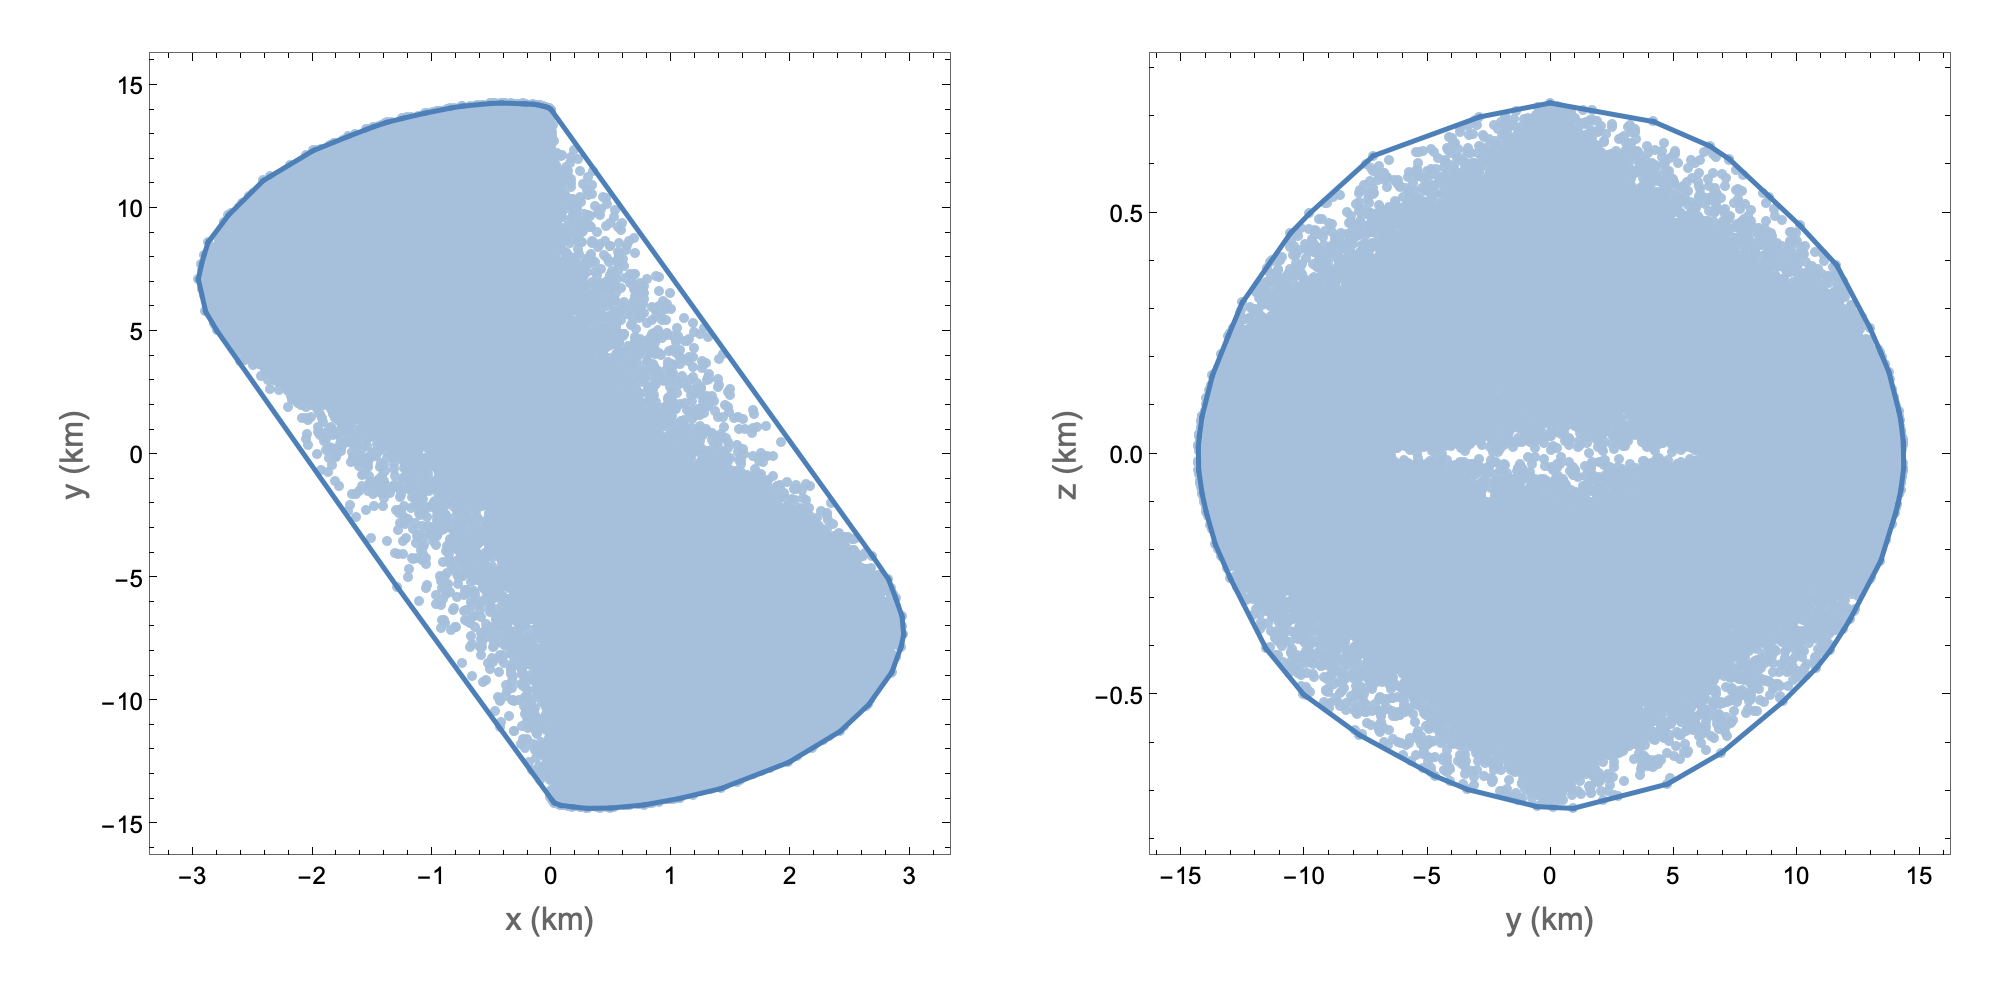
\includegraphics[width=\columnwidth]{2pilinear.png}
    \caption{Multi impulse reachable set for linear dynamics, projected onto the $x$--$y$ plane (left) and the $y$--$z$ plane (right).}
    \label{fig:2pi-linear}
\end{figure}

Figure~\ref{fig:2pi-nonlinear} shows the corresponding example for nonlinear dynamics.

\begin{figure}[htbp]
    \centering
    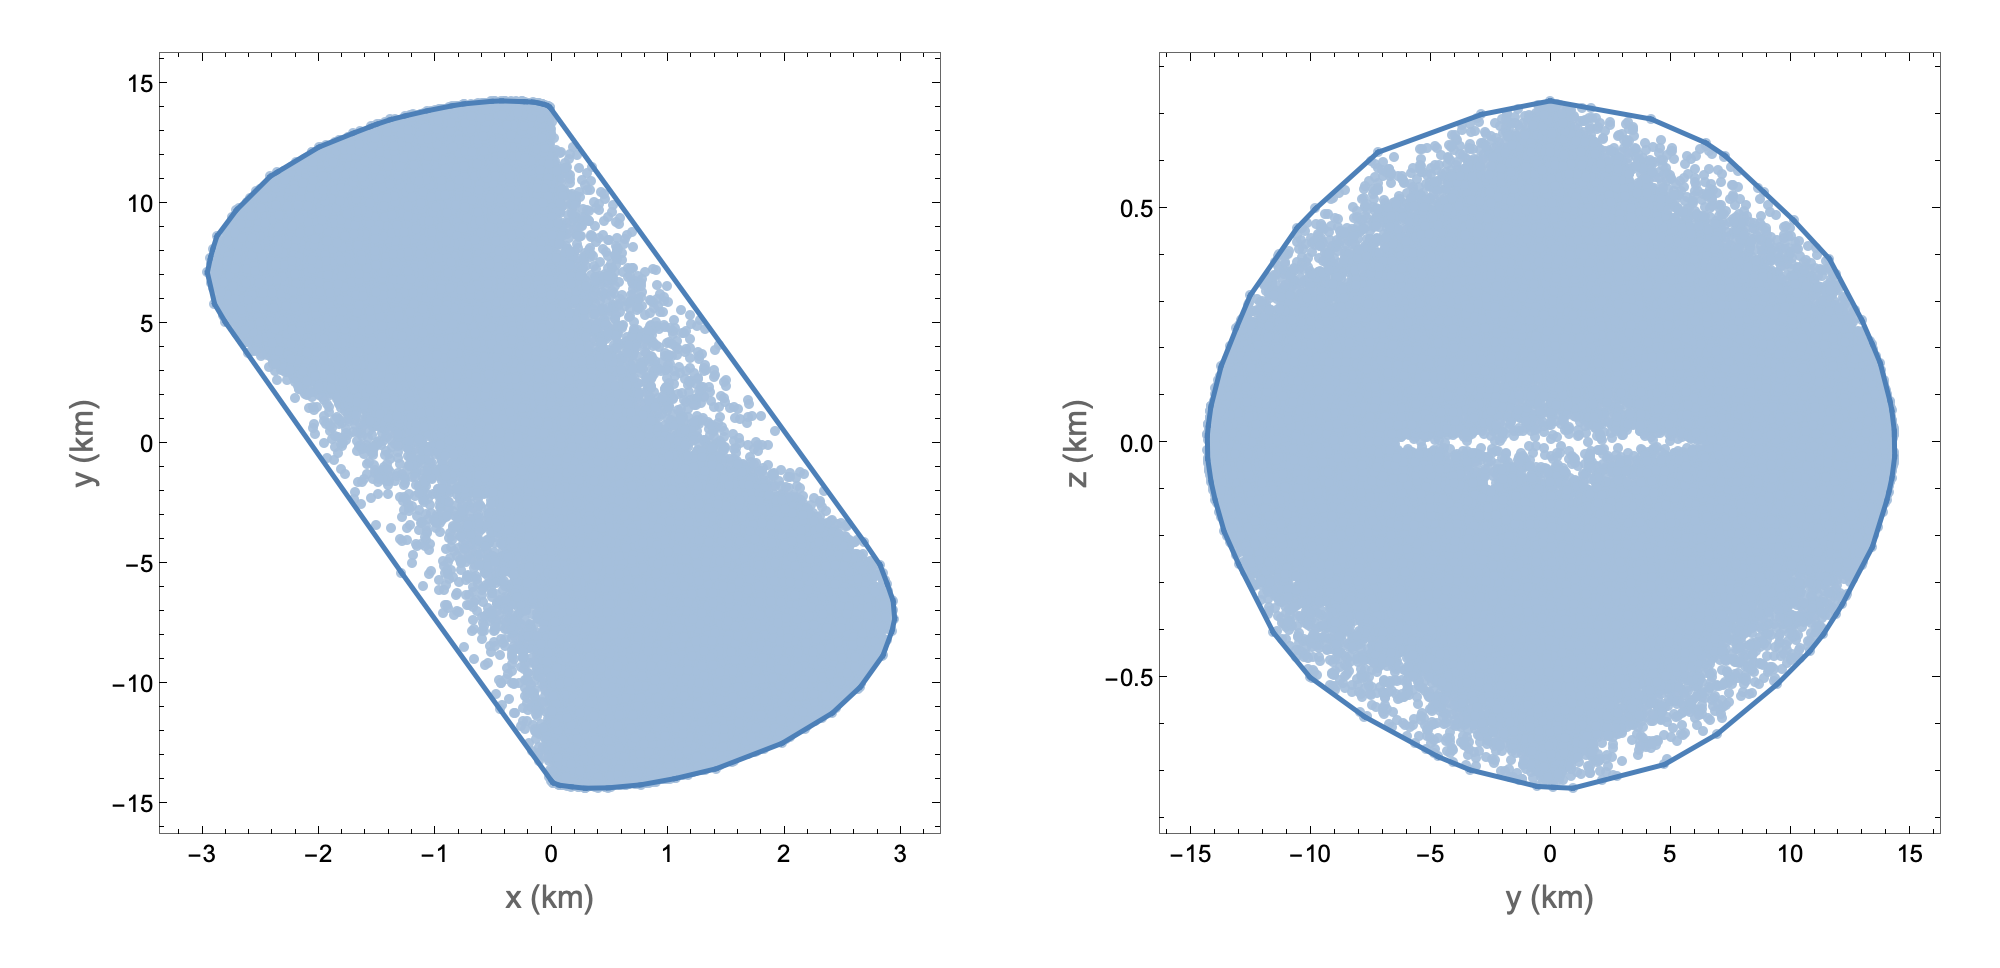
\includegraphics[width=\columnwidth]{2pinonlinear.png}
    \caption{Multi impulse reachable set for nonlinear dynamics, projected onto the $x$--$y$ plane (left) and the $y$--$z$ plane (right).}
    \label{fig:2pi-nonlinear}
\end{figure}

Figure~\ref{fig:ratios} compares the nonlinear and linear reachable-set extents as a function of projection angle. The flight parameters used for this comparison were deliberately selected to stress-test the algorithm. Because larger available $\Delta v$ produces greater separation from the reference trajectory, the nonlinear dynamics depart more strongly from the linear approximation; this case therefore emphasizes the differences between the two reachable sets.

\begin{figure}[htbp]
    \centering
    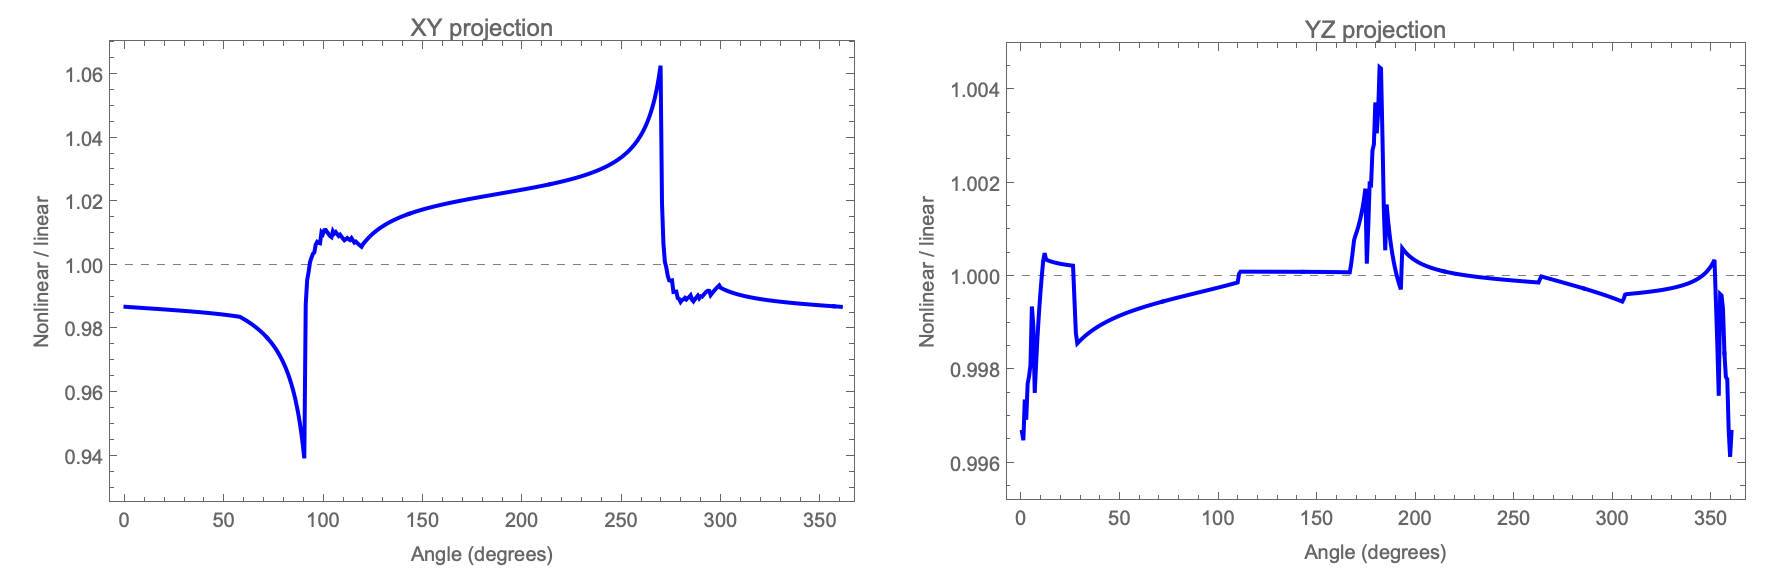
\includegraphics[width=\columnwidth,trim=0 0 445.163pt 0,clip]{samplecomparison.png}
    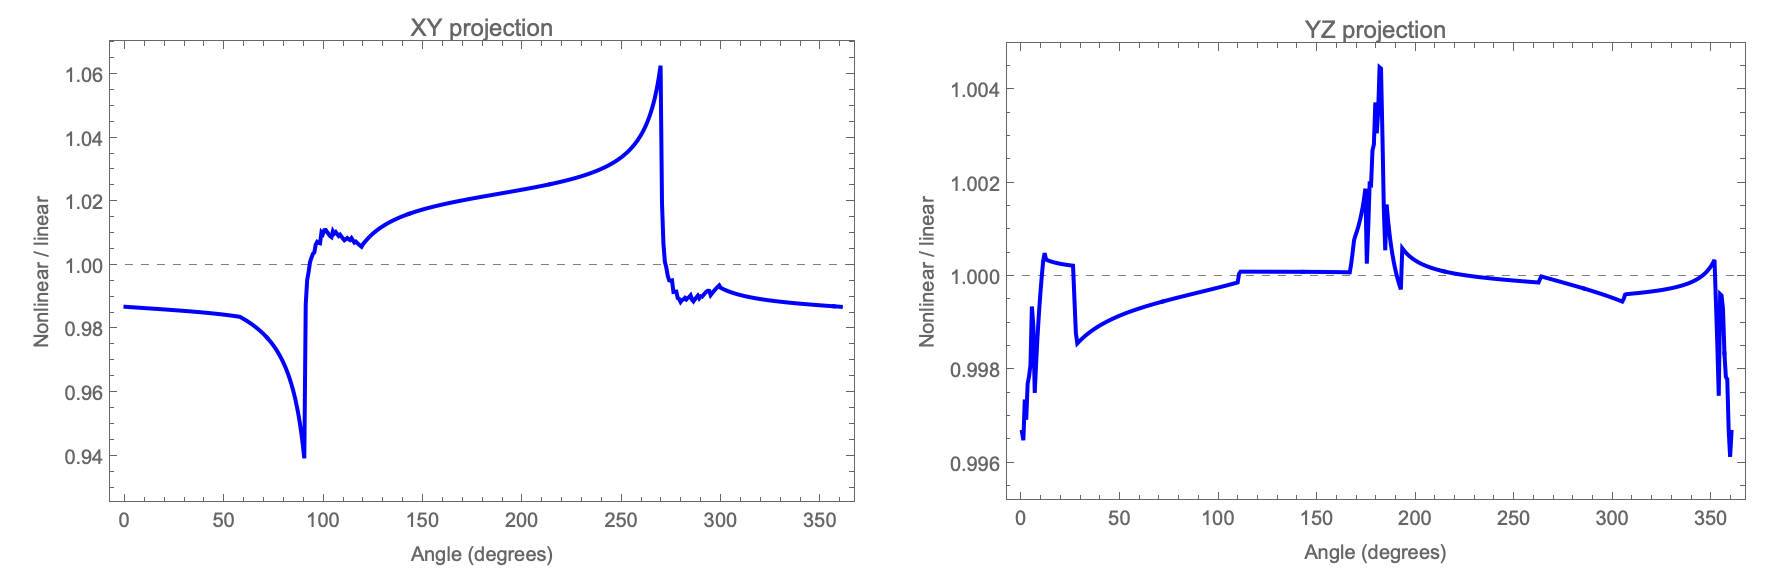
\includegraphics[width=\columnwidth,trim=426.594pt 0 0 0,clip]{samplecomparison.png}
    \caption{Angular comparison of the nonlinear and linear reachable-set extents in the $x$--$y$ projection (top) and the $y$--$z$ projection (bottom). The plotted quantity is the ratio of the nonlinear extent to the linear extent at each angle.}
    \label{fig:ratios}
\end{figure}


\section{CONCLUSIONS}
We have designed a sampling-based algorithm for computation of multi-impulse reachable sets. The algorithm was tested on linear and non-linear two-body relative motion equations. We have demonstrated that the algorithm is computationally tractable for linear systems with three position and three velocity variables, as well as for non-linear systems for which a limited number of impulses are required. To facilitate our studies, first we proved an analog to Prussing's sufficiency result that is specific to our case, and then we extended Prussing's sufficiency proof to impulsive linear systems with convex terminal objectives and constraint sets. Finally, we presented numerical examples of the multi-impulse reachable set, comparing them to  

%%%%%%%%%%%%%%%%%%%%%%%%%%%%%%%%%%%%%%%%%%%%%%%%%%%%%%%%%%%%%%%%%%%%%%%%%%%%%%%%



%%%%%%%%%%%%%%%%%%%%%%%%%%%%%%%%%%%%%%%%%%%%%%%%%%%%%%%%%%%%%%%%%%%%%%%%%%%%%%%%



%%%%%%%%%%%%%%%%%%%%%%%%%%%%%%%%%%%%%%%%%%%%%%%%%%%%%%%%%%%%%%%%%%%%%%%%%%%%%%%%

\section*{ACKNOWLEDGMENT}

The preferred spelling of the word ÒacknowledgmentÓ in America is without an ÒeÓ after the ÒgÓ. Avoid the stilted expression, ÒOne of us (R. B. G.) thanks . . .Ó  Instead, try ÒR. B. G. thanksÓ. Put sponsor acknowledgments in the unnumbered footnote on the first page.



%%%%%%%%%%%%%%%%%%%%%%%%%%%%%%%%%%%%%%%%%%%%%%%%%%%%%%%%%%%%%%%%%%%%%%%%%%%%%%%%


\bibliography{citations}


\end{document}
